\documentclass[a4paper]{report}

\usepackage{amssymb, amsmath}
\usepackage{tikz}

\newcommand{\vens}{\ensuremath{v_{\mathrm{ens}}}}


\title{Replicating John Philip 1972}
\author{Nat Lund}

\begin{document}
\maketitle

Rough working as we attempt to replicate the double Schwarz-Christoffel transformations in J.\ R.\ Philip's 1972 paper in ZAMP.

We map:
\begin{center}
\begin{tikzpicture}

\draw[thick] (-2,3) -- (-2,0) -- (0,0) -- (2,0) -- (2,3);
\draw[fill] (-2,0) circle (0.5mm) node[below]{$-b$}
            (-1,0) circle (0.5mm) node[below]{$-a$}
            (0,0)  circle (0.5mm) node[below]{$0$}
            (1,0)  circle (0.5mm) node[below]{$a$}
            (2,0)  circle (0.5mm) node[below]{$b$};
\node at (0,3) {$\mathbb{C}$};

\coordinate (orig) at (6,0);
\node at (3,1.5) {to};

\draw[thick] (orig) ++(-2,3) -- ++(0,-3) -- ++(4,0) -- ++(0,3) (orig) -- ++(0,1.5);
\draw[fill] (orig)           circle (0.5mm) node[below]{$0$} 
            (orig) ++(-2,0)  circle (0.5mm) node[below]{$-b$}
            (orig) ++(2,0)   circle (0.5mm) node[below]{$b$}
            (orig) ++(0,1.5) circle (0.5mm) node[right]{$ic$};

\node at (6,3) {$\mathbb{C}_1$};

\end{tikzpicture}
\end{center}

presumably via the upper half plane $\mathbb{H}$:
\vspace*{1em}

\begin{center}
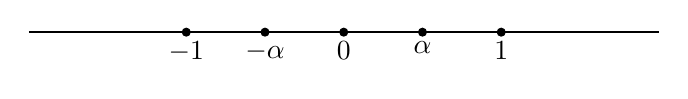
\begin{tikzpicture}

\draw[thick] (-4,0) -- (4,0);
\draw[fill] (-2,0) circle (0.5mm)  node[below]{$-1$} 
            (-1,0) circle (0.5mm)  node[below]{$-\alpha$}
            (0,0)  circle (0.5mm)  node[below]{$0$}
            (1,0)  circle (0.5mm)  node[below]{$\alpha$}
            (2,0)  circle (0.5mm)  node[below]{$1$};


\end{tikzpicture}
\end{center}

where $\displaystyle \alpha = \frac{a}{b}$

\vspace*{1em}
The Schwarz-Christoffel mapping from $\mathbb{H}$ to $\mathbb{C}_1$ should be given by the indefinite integral:
\begin{equation}
z = \int \frac{w}{\sqrt{w^2 - 1} \sqrt{w^2 - \alpha^2}}
\end{equation}
which according to Wolfram's online Integrator, has solution:
\begin{equation}
z = \ln \left( 2  \sqrt{w^2 - 1} + 2 \sqrt{w^2 - \alpha^2} \right)
\end{equation}
The factor of 2 can be pulled out into $C$:
\begin{equation}
z = K \ln \left( \sqrt{w^2 - 1} + \sqrt{w^2 - \alpha^2} \right) + C
\end{equation}


Let us check:
\begin{gather*}
\frac{d}{dw} \ln \left( \sqrt{w^2 - 1} + \sqrt{w^2 - \alpha^2} \right) = 
\frac{ \frac{d}{dw} \left( \sqrt{w^2 - 1} + \sqrt{w^2 - \alpha^2} \right) }
     { \sqrt{w^2 - 1} + \sqrt{w^2 - \alpha^2} } \\
= \frac{ \frac{2w}{2 \sqrt{w^2 -1}} + \frac{2w}{2 \sqrt{w^2 - \alpha^2}} }
       { \sqrt{w^2 - 1} + \sqrt{w^2 - \alpha^2} }
= \frac{ w \left( \frac{1}{\sqrt{w^2 -1}} + \frac{1}{\sqrt{w^2 - \alpha^2}} \right) }
       { \sqrt{w^2 - 1} + \sqrt{w^2 - \alpha^2} } \\
= \frac{ w \left( \frac{\sqrt{w^2 - 1} + \sqrt{w^2 - \alpha^2}}
                       {\sqrt{w^2 - 1}\sqrt{w^2 - \alpha^2}}  \right) }
       {\sqrt{w^2 - 1} + \sqrt{w^2 - \alpha^2}}
= \frac{w}{\sqrt{w^2 - 1}\sqrt{w^2 - \alpha^2}} \quad \text{tick!}
\end{gather*}

\end{document}
